\documentclass[11pt]{article}
\usepackage[margin=1in]{geometry}
\usepackage[T1]{fontenc}
\usepackage{amsmath,amssymb,amsthm}
\usepackage{graphicx}
\usepackage{booktabs}
\usepackage[numbers,sort&compress]{natbib}
\usepackage{xcolor}
\usepackage{hyperref}
\usepackage{xurl}
\hypersetup{colorlinks=true,linkcolor=black,citecolor=black,urlcolor={rgb:red,0.1;green,0.3;blue,0.6}}
\usepackage{microtype}

\newtheorem{theorem}{Theorem}
\newtheorem{proposition}{Proposition}
\newtheorem{lemma}{Lemma}
\newtheorem{corollary}{Corollary}
\renewcommand{\topfraction}{0.9}
\renewcommand{\textfraction}{0.1}
\renewcommand{\floatpagefraction}{0.8}
\newcommand{\T}{\mathsf{T}}
\newcommand{\Bx}{\mathcal{B}}
\newcommand{\lP}{\lambda_{\mathrm{P}}}

\title{Signed Kekul\'e structures and H\"uckel gap-closure thresholds in phenylenes}
\author{Xiyao Yu\thanks{ORCID: \href{https://orcid.org/0009-0006-2673-5269}{0009-0006-2673-5269}. Email: \href{mailto:XYU029@e.ntu.edu.sg}{XYU029@e.ntu.edu.sg}}\\[2pt]
{\small School of Chemistry, Chemical Engineering and Biotechnology,}\\
{\small Nanyang Technological University, Singapore}}
\date{}

\begin{document}
\maketitle

\begin{abstract}
The HOMO--LUMO gap is a fundamental descriptor of molecular electronic structure, but its size alone does not reveal how resistant it is to changes in bonding. In H\"uckel theory, electronic interactions between bonded carbon atoms are represented by coupling parameters. Changes in these couplings, such as those arising from bond-length distortions, shift the orbital energies and can eventually bring the HOMO and LUMO together, closing the gap. Surprisingly, a molecule with a smaller initial gap may require larger changes to reach this point. What, then, determines how robust a gap is?

Here we introduce the gap-closure threshold, the smallest bound on the relative change of the bond couplings that permits the gap to close without altering the molecular connectivity. For equal reference couplings, this threshold is determined entirely by the Kekul\'e structures of the carbon skeleton together with their signs. It reaches its maximum exactly when all Kekul\'e structures have the same sign, and it can be obtained analytically when only one structure has the minority sign. For other skeletons, it lies between lower bounds that each require one eigenvalue computation and an upper bound obtained from a single minority structure. For phenylenes, skeletons with the same sequence of linear and angular annelations share an identical threshold, even when their electronic spectra differ. How the change is distributed over the bonds matters as well: in biphenylene, coordinated changes of 18.9\% in all couplings close the gap, whereas a single coupling must increase by 300\%. Across nine skeletons, the threshold also ranks the energies required for gap closure in a bond-length model more accurately than the gap of the relaxed geometry does (Spearman correlations of 0.94 and 0.72).

These results establish a quantitative distinction between the magnitude and the robustness of molecular electronic gaps, and show how robustness can be understood through the combinatorial structure of chemical bonding.
\end{abstract}

\noindent\textbf{Keywords:} H\"uckel theory; Kekul\'e structures; algebraic structure count; sign-nonsingular matrices; regularity radius; isoarithmicity; phenylenes

\noindent\textbf{Mathematics Subject Classification (2020):} 92E10; 05C92; 05C70; 15A15; 15B35; 65G40

% =====================================================================
\section{Introduction}

In H\"uckel theory, the $\pi$ orbitals of a conjugated hydrocarbon are the eigenvectors of a matrix with one row and one column for each carbon atom and a nonzero entry, the coupling, for each carbon--carbon bond (Fig.~\ref{fig:bcb}a,\,b). When all couplings are equal, this matrix is a multiple of the adjacency matrix of the molecular graph, whose vertices are the carbon atoms and whose edges are the bonds. The orbital energies are then determined by the eigenvalues of the graph, and questions about orbitals become questions about graphs \citep{GutmanPolansky1986,CvetkovicDoobSachs1980}. The HOMO--LUMO gap, the energy difference between the highest occupied and the lowest unoccupied orbital, is one such quantity, and how it depends on the structure of the graph has been studied directly \citep{GutmanRouvray1979,FowlerPisanski2010}.

In an alternant hydrocarbon the carbon atoms fall into two sets, starred and unstarred, and every bond joins atoms of different sets. When the two sets have the same size $n$, the H\"uckel matrix is determined by the $n\times n$ matrix $T$ of couplings between them (Fig.~\ref{fig:bcb}b). The orbital energies come in pairs $\pm\sigma_k(T)$, where $\sigma_k(T)$ are the singular values of $T$, and the HOMO and LUMO lie at $-\sigma_{\min}(T)$ and $+\sigma_{\min}(T)$. The gap $2\sigma_{\min}(T)$ is therefore zero, with HOMO and LUMO degenerate at zero energy, exactly when $\det T=0$. We say that the gap \emph{closes}.

\begin{figure}[tb]
\centering
\begin{minipage}[c]{0.34\textwidth}\centering
{\small\textbf{a}}\\[1pt]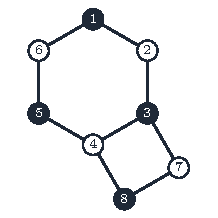
\includegraphics{fig_bcb_graph.pdf}
\end{minipage}\hfill
\begin{minipage}[c]{0.64\textwidth}\centering
{\small\textbf{b}}\\[3pt]
$\displaystyle H=-\begin{pmatrix}0&T\\ T^{\T}&0\end{pmatrix}$\\[6pt]
$\displaystyle T=\begin{pmatrix}t_{12}&0&t_{16}&0\\ t_{23}&t_{34}&0&t_{37}\\ 0&t_{45}&t_{56}&0\\ 0&t_{48}&0&t_{78}\end{pmatrix}$
\end{minipage}\\[8pt]
{\small\textbf{c}}\\[1pt]
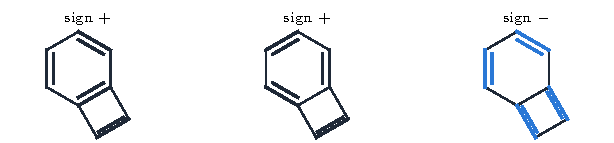
\includegraphics{fig_bcb_kekule.pdf}\\[3pt]
$\det T=t_{12}t_{34}t_{56}t_{78}+t_{16}t_{23}t_{45}t_{78}-t_{12}t_{37}t_{48}t_{56}$
\caption{From carbon skeleton to matrix, for benzocyclobutadiene. (a) The molecular graph: one vertex for each carbon atom and one edge for each bond. Starred atoms (1, 3, 5, 8) are black, unstarred atoms (2, 4, 6, 7) white, and every bond joins a black and a white atom. (b) The H\"uckel matrix with Coulomb integrals set to zero and the starred atoms listed first. It is determined by the matrix $T$ of couplings $t_{ij}$, whose rows are the starred atoms 1, 3, 5, 8 and whose columns are the unstarred atoms 2, 4, 6, 7. (c) The three Kekul\'e structures and the expansion of $\det T$: each structure contributes the product of the couplings of its double bonds, with the sign shown. At equal couplings $\det T=1+1-1=1$.}
\label{fig:bcb}
\end{figure}

A Kekul\'e structure places double bonds so that every carbon atom lies in exactly one of them. At equal couplings, $\det T$ is a signed count of these structures (Fig.~\ref{fig:bcb}c). Two structures carry opposite signs when they differ around an odd number of cycles of length $4k$ \citep{DewarLH1952}, and $|\det T|$ is the algebraic structure count \citep{Wilcox1968,Wilcox1969}. In benzenoid hydrocarbons all Kekul\'e structures carry the same sign, so the terms of $\det T$ cannot cancel: whatever positive values the couplings take, $\det T\neq0$ and the gap stays open. Combinatorial matrix theory calls a pattern of zero and positive entries with this property sign-nonsingular \citep{BrualdiShader1995}. Phenylenes, which alternate six- and four-membered rings, have structures of both signs. Their algebraic structure count equals the Kekul\'e structure count of the hexagonal squeeze \citep{Gutman1993}, and for unbranched hexagonal chains that count depends only on the sequence of linear and angular annelations, a property known as isoarithmicity \citep{GordonDavison1952,BalabanTomescu1983}. The algebraic structure count entered chemical graph theory as a stability index. Wilcox related it to the stability of hydrocarbons with four-membered rings \citep{Wilcox1968,Wilcox1969}, and a count of zero, which means a closed gap, marks a hydrocarbon expected to be extremely reactive \citep{BodrozaPantic2007}. Recurrences \citep{BodrozaPantic2004,BodrozaPantic2007} and rigorous bounds on H\"uckel properties \citep{FowlerPickup2024} have since extended what can be computed from the graph. As a stability index, however, the count is evaluated at equal couplings, whereas in a molecule substituents, strain and bond-length alternation change the couplings bond by bond and can push it toward the small gaps associated with open-shell, diradical character \citep{MolesQuintero2022}. A nonzero count says that the gap is open at equal couplings; it does not say how robust the open gap is. Biphenylene and naphthalene, for example, both have count three. The gap of naphthalene stays open for all positive couplings, whereas that of biphenylene closes once each coupling has changed by 18.9\%. A graph invariant that measures how far the couplings of a skeleton must move before its gap closes would turn the zero/nonzero criterion into a quantitative one. This paper defines such an invariant and shows how to compute it from the signed Kekul\'e structures.

To make the question precise, we keep the set of bonds fixed and allow each coupling to change by up to a fixed fraction of its value, for example by up to 10\%. We ask for the smallest fraction at which some choice of changes closes the gap, and which features of the signed Kekul\'e structures determine it. Biphenylene shows that the answer depends on how the change is distributed over the bonds (Fig.~\ref{fig:hook}). If only one coupling may change, the gap closes only when the coupling of one of the two bonds joining the benzene rings is multiplied by four, an increase of 300\%. If all fourteen couplings may change, some up and some down, the gap closes once each has changed by 18.9\%. One might expect the size of the gap to predict this fraction, with smaller gaps being easier to close. It does not. Angular [3]phenylene has a smaller gap than biphenylene (0.844 against $0.890\,|\beta|$) but needs a larger change, and helical and zigzag [4]phenylene have different gaps but need exactly the same change (Table~\ref{tab:rho}). Section~\ref{sec:model} shows that the gap is itself a distance to singularity, but one that allows bonds to be created; the question here concerns the skeleton as it is.

\begin{figure}[t]
\centering
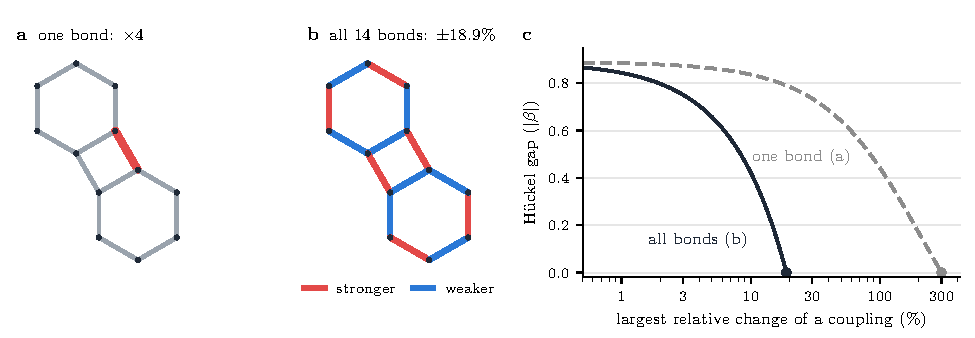
\includegraphics{fig1_hook.pdf}
\caption{Closing the H\"uckel gap of biphenylene. (a) The smallest single-bond change: the coupling of the red bond must grow from 1 to 4. (b) The smallest change of all couplings: red couplings grow and blue couplings shrink, each by 18.9\%. (c) The gap along both paths; the horizontal axis is the largest relative change of any coupling.}
\label{fig:hook}
\end{figure}

This paper gives the following answers. (i) We define the closure threshold $\rho$, identify it with the regularity radius of an interval matrix \citep{PoljakRohn1993,HartmanHladik2018}, and show that $\rho=1$ exactly for sign-nonsingular patterns and that $\rho$ depends only on the signed Kekul\'e structures (Section~\ref{sec:model}). (ii) When exactly one Kekul\'e structure carries the less frequent sign, $\rho$ is the root of a polynomial equation in the numbers of bonds by which the other structures differ from it, and the change that attains it is explicit. For general skeletons, strengthening the bonds of one such structure gives an upper bound, and known spectral conditions for interval matrices give lower bounds (Section~\ref{sec:one}). (iii) A gluing formula for the signed Kekul\'e polynomial shows that phenylenes with the same sequence of linear and angular annelations have the same signed Kekul\'e polynomial up to a relabelling of bonds, and hence the same threshold (Section~\ref{sec:la}). (iv) For the [$N$]phenylenes with $N\le4$ we compute $\rho$ exactly, certify each value and list every change that attains it; for $N=5$ and 6 we bracket it (Section~\ref{sec:phenylenes}). (v) As an application, $\rho$ ranks the energies needed to close the gap in a bond-length model (Section~\ref{sec:energy}).

% =====================================================================
\section{Signed Kekul\'e structures and gap closure}
\label{sec:model}

We use the H\"uckel model of an alternant hydrocarbon with $2n$ carbon atoms, $n$ in each of the two sets (starred and unstarred). With Coulomb integrals set to zero and couplings $t_{ij}=-\beta_{ij}>0$ between bonded atoms $i$ (starred) and $j$ (unstarred), the Hamiltonian is
\begin{equation}
H=-\begin{pmatrix}0&T\\T^\T&0\end{pmatrix},
\end{equation}
where $T$ is the $n\times n$ matrix of couplings. The orbital energies are $\pm\sigma_k(T)$, the singular values of $T$, so the gap is
\begin{equation}
g=2\,\sigma_{\min}(T),
\end{equation}
and it closes exactly when $\det T=0$. All couplings equal one unless stated; energies are in units of $|\beta|$. We write $m$ for the number of bonds.

\textbf{The determinant counts Kekul\'e structures with signs.} Expanding $\det T$ gives one term for each Kekul\'e structure, that is, each set of bonds that covers every atom exactly once:
\begin{equation}
\det T=\sum_{M}s_M\prod_{(ij)\in M}t_{ij},\qquad s_M=\pm1 .
\label{eq:expansion}
\end{equation}
We call the right side, viewed as a polynomial in one variable per bond, the \emph{signed Kekul\'e polynomial} of the skeleton; it is defined up to an overall sign, which depends on the order of rows and columns. We fix this sign so that $\det T>0$ at the couplings considered, and call a structure with $s_M=-1$ a \emph{minority structure}. At equal couplings $\det T$ is the number of structures of sign $+$ minus the number of sign $-$, so the minority structures are the less numerous ones. Benzenoid hydrocarbons have none. A four-membered ring creates them, because two structures that differ only by the positions of the double bonds around a four-membered ring have opposite signs \cite{DewarLH1952}. Benzocyclobutadiene has two structures of sign $+$ and one of sign $-$ (Fig.~\ref{fig:bcb}c), so its algebraic structure count is $2-1=1$; biphenylene has four and one, and count 3.

One further property of Eq.~\eqref{eq:expansion} is used repeatedly below. A Kekul\'e structure contains each bond at most once, so each term contains a given coupling $t_{ij}$ at most to the first power. With all other couplings fixed, $\det T$ is therefore a function of the form $\alpha+\beta\,t_{ij}$: it is affine in each coupling separately.

\textbf{The closure threshold.} For $\epsilon\ge0$ let $\Bx_\epsilon(T)$ be the set of matrices $T'$ with $T'_{ij}=0$ wherever $T_{ij}=0$ and $|T'_{ij}-T_{ij}|\le\epsilon\,T_{ij}$ otherwise: every coupling may change by the fraction $\epsilon$ of its value, and no bond is created or removed. The \emph{gap-closure threshold} of the skeleton, or closure threshold for short, is
\begin{equation}
\rho=\min\bigl\{\epsilon\ge0:\ \Bx_\epsilon(T)\ \text{contains a singular matrix}\bigr\}.
\label{eq:rho}
\end{equation}
The set $\Bx_\epsilon(T)$ is the interval matrix $[T-\epsilon T,\,T+\epsilon T]$, and $\rho$ is its regularity radius, the smallest $\epsilon$ at which the interval matrix contains a singular matrix \citep{PoljakRohn1993,Rohn2009,HartmanHladik2018}; in numerical linear algebra the same quantity is the componentwise distance of $T$ to the nearest singular matrix, relative to $|T|$ \citep{Rump1999}. For general matrices it is NP-hard to compute \citep{PoljakRohn1993}. The threshold is a continuous, signed counterpart of the anti-Kekul\'e number, the smallest number of bonds whose removal leaves a connected graph without Kekul\'e structures \citep{Hayat2021}: there bonds are deleted and every structure disappears, here couplings change and structures of opposite sign cancel.

\textbf{The gap is also a distance to singularity.} By the Eckart--Young theorem \citep{EckartYoung1936},
\[
\sigma_{\min}(T)=\min\bigl\{\|E\|_2:\ T+E\ \text{is singular}\bigr\},
\]
where $\|E\|_2$ is the spectral norm and $E$ ranges over all $n\times n$ matrices. Such an $E$ may put nonzero entries where $T$ has zeros, that is, create a bond between any starred and any unstarred atom, and it measures the change in absolute rather than relative terms. The half-gap $g/2$ and the threshold $\rho$ therefore measure the distance from $T$ to the same set of singular matrices, under different rules. The gap admits perturbations that no change of bond lengths can produce; $\rho$ admits only changes of the existing couplings. This is why the two can order skeletons differently. The closure energy of Section~\ref{sec:energy} is, in its local approximation, a third version of the same distance: changes restricted to the existing bonds, measured in a weighted Euclidean norm of the bond-length changes.

\begin{lemma}
\label{lem:range}
Let $T$ have positive couplings on its bonds and $\det T\neq0$. Then $0<\rho\le1$, and the following are equivalent:
\begin{enumerate}
\item[(a)] $\rho=1$;
\item[(b)] the zero pattern of $T$ is sign-nonsingular, that is, every matrix with positive entries exactly on the bonds is nonsingular;
\item[(c)] all Kekul\'e structures carry the same sign.
\end{enumerate}
\end{lemma}

\begin{proof}
$\rho>0$ because $\det$ is continuous and $\Bx_0(T)=\{T\}$. At $\epsilon=1$ the box contains the zero matrix, so $\rho\le1$. (c)$\Rightarrow$(b): every term of Eq.~\eqref{eq:expansion} has the same sign for all positive couplings. (b)$\Rightarrow$(a): for $\epsilon<1$ every matrix in $\Bx_\epsilon(T)$ has positive entries exactly on the bonds. (a)$\Rightarrow$(c): suppose a minority structure $M'$ exists. Set the couplings of its bonds to $(1+\epsilon)t_{ij}$ and all others to $(1-\epsilon)t_{ij}$. Every positive term contains a bond outside $M'$ and tends to zero as $\epsilon\to1$, while the term of $M'$ tends to $-2^n\prod_{M'}t_{ij}$ and the remaining terms are negative. The determinant is therefore negative for some $\epsilon<1$ and vanishes in between, so $\rho<1$.
\end{proof}

Benzene and naphthalene therefore have $\rho=1$. For a pattern that is not sign-nonsingular, $\rho<1$ measures, in relative terms, how close to $T$ the sign freedom that sign-nonsingularity excludes produces a singular matrix.

\begin{proposition}
\label{prop:inv}
Let two skeletons with equal couplings have the same number $m$ of bonds, and suppose a one-to-one correspondence of their bonds turns the signed Kekul\'e polynomial of one into that of the other, up to an overall sign. Then the two skeletons have the same closure threshold.
\end{proposition}

\begin{proof}
With equal couplings, $\Bx_\epsilon(T)$ is the cube $[1-\epsilon,1+\epsilon]^m$ in the bond variables. The correspondence permutes the variables and maps this cube onto the cube of the other skeleton, and it carries the zeros of one determinant onto the zeros of the other. Both skeletons therefore contain a singular matrix in their box for the same values of $\epsilon$.
\end{proof}

Proposition~\ref{prop:inv} rests on two observations. First, $\rho$ is defined through $\det T$ alone: Eq.~\eqref{eq:rho} asks only whether some matrix in the box has determinant zero. Second, $\det T$ is the signed Kekul\'e polynomial, so it is fixed by the list of Kekul\'e structures, each viewed as a set of bonds, together with their signs. A correspondence of bonds that carries this list for one skeleton onto the list for the other therefore carries one determinant onto the other, and with it the threshold. The gap behaves differently. It equals $2\sigma_{\min}(T)$, and the singular values of $T$ depend on where the couplings sit in the matrix, not only on its determinant. Two skeletons related as in Proposition~\ref{prop:inv} can therefore have different gaps and the same threshold. Section~\ref{sec:la} shows that this happens throughout the phenylenes; helical and zigzag [4]phenylene are the smallest example.

% =====================================================================
\section{Minority structures and two-sided bounds}
\label{sec:one}

\subsection{One minority structure}

In this section we compute $\rho$ for the simplest skeletons that are not sign-nonsingular: those with exactly one minority structure $M_-$, such as benzocyclobutadiene and biphenylene. At equal couplings $\det T$ is then a sum of $K-1$ positive terms and one negative term, and it vanishes when the negative term catches up with the positive ones. What matters is the ratio of each positive term to the negative one. Couplings shared by a positive term and $M_-$ cancel in this ratio; the remaining couplings of the positive term lie outside $M_-$, and the remaining couplings of $M_-$ lie outside the positive term. Increasing every coupling of $M_-$ and decreasing every other coupling therefore lowers all ratios at once. Theorem~\ref{thm:one} shows that no other change of the same size does better, and turns this choice into an equation for $\rho$.

\begin{theorem}
\label{thm:one}
Let a skeleton with equal couplings have $K$ Kekul\'e structures and $\det T\neq0$. Suppose exactly one structure, $M_-$, has the minority sign, and let $M_1,\dots,M_{K-1}$ be the others. Let $k_a=|M_a\setminus M_-|$ be the number of bonds in which $M_a$ differs from $M_-$. Then
\begin{equation}
\rho=\frac{1-q}{1+q},\qquad\text{where $q$ is the unique root in $(0,1)$ of}\quad \sum_{a=1}^{K-1}q^{k_a}=1 .
\label{eq:closedform}
\end{equation}
The threshold is attained by setting the coupling of every bond of $M_-$ to $1+\rho$ and every other coupling to $1-\rho$. If every bond belongs to at least one, but not to every, Kekul\'e structure, this is the only singular matrix in $\Bx_\rho(T)$.
\end{theorem}

\begin{proof}
At equal couplings $\det T=K-2>0$, so $K-1\ge2$, and the left side of Eq.~\eqref{eq:closedform} increases strictly from 0 to $K-1$ on $[0,1]$, which makes the root unique. Divide Eq.~\eqref{eq:expansion} by the term of $M_-$. Bonds shared by $M_a$ and $M_-$ cancel, so
\begin{equation}
\frac{\det T}{\prod_{M_-}t_{ij}}=\sum_{a=1}^{K-1}r_a-1,\qquad
r_a=\frac{\prod_{(ij)\in M_a\setminus M_-}t_{ij}}{\prod_{(ij)\in M_-\setminus M_a}t_{ij}} .
\end{equation}
Both products contain $k_a$ couplings. With every coupling in $[1-\epsilon,1+\epsilon]$ and $q=(1-\epsilon)/(1+\epsilon)$, each $r_a\ge q^{k_a}$, with equality exactly when the couplings in the numerator equal $1-\epsilon$ and those in the denominator equal $1+\epsilon$. The setting of the theorem makes this true for every $a$ at once, so the smallest value of $\sum_ar_a$ over $\Bx_\epsilon(T)$ is $\sum_aq^{k_a}$. The largest value is at least $K-1>1$, and the box is connected, so $\Bx_\epsilon(T)$ contains a singular matrix exactly when $\sum_aq^{k_a}\le1$. This gives Eq.~\eqref{eq:closedform}.

It remains to prove uniqueness. Let $\epsilon=\rho$, so that $\sum_aq^{k_a}=1$, and let $T'$ be a singular matrix in $\Bx_\rho(T)$. Then $\sum_ar_a=1$ at $T'$. Each $r_a$ is at least $q^{k_a}$, and these lower bounds already sum to 1, so every $r_a$ equals its lower bound. By the equality condition above, every coupling that appears in the numerator of some $r_a$ equals $1-\rho$, and every coupling that appears in the denominator of some $r_a$ equals $1+\rho$. Now take any bond $e$. If $e$ belongs to $M_-$ but not to some $M_a$, it appears in the denominator of $r_a$, so its coupling is $1+\rho$. If $e$ does not belong to $M_-$ but belongs to some $M_a$, it appears in the numerator of $r_a$, so its coupling is $1-\rho$. A bond that fits neither case belongs either to every Kekul\'e structure or to none, and the condition of the theorem excludes both. Every coupling of $T'$ is therefore determined, and $T'$ is the matrix described in the theorem.
\end{proof}

\begin{figure}[t]
\centering
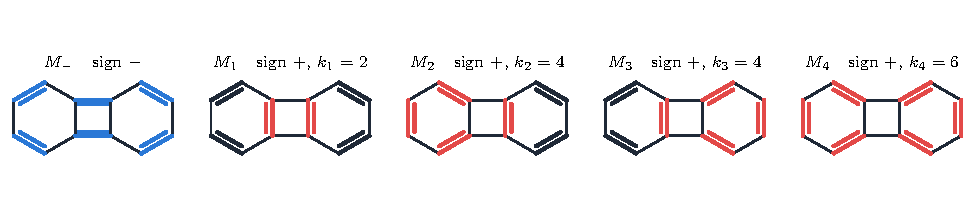
\includegraphics{fig_kekule.pdf}
\caption{The five Kekul\'e structures of biphenylene. $M_-$ (blue) is the only minority structure; both bonds joining the benzene rings are double in it. In $M_1,\dots,M_4$ the double bonds that $M_-$ does not contain are red; their number is $k_a$. Theorem~\ref{thm:one} turns the exponents $2,4,4,6$ into $q^2+2q^4+q^6=1$, that is, $q^3+q=1$.}
\label{fig:kekule}
\end{figure}

\textbf{Benzocyclobutadiene.} The minority structure has double bonds on both bonds that join the four-membered ring to the rest of the molecule. The two other structures differ from it around the four-membered ring (two bonds) and around the eight-membered perimeter (four bonds), so $q^2+q^4=1$, $q^2=1/\varphi$ with $\varphi$ the golden ratio, and
\begin{equation}
\rho_{\text{BCB}}=\frac{\sqrt{\varphi}-1}{\sqrt{\varphi}+1}=0.11973 .
\end{equation}

\textbf{Biphenylene.} The minority structure $M_-$ has both bonds joining the benzene rings double, so that each benzene ring keeps only two double bonds (Fig.~\ref{fig:kekule}). The four other structures differ from it in 2, 4, 4 and 6 bonds: one flips the four-membered ring, two flip one benzene ring each together with the four-membered ring, and one flips both benzene rings. Hence $q^2+2q^4+q^6=q^2(1+q^2)^2=1$, which reduces to
\begin{equation}
q^3+q=1,\qquad q=0.68233,\qquad \rho_{\text{biphenylene}}=0.18883 .
\end{equation}
In both molecules every bond belongs to some but not all Kekul\'e structures, so the closing change is unique: in biphenylene the six bonds of $M_-$ grow by 18.9\% and the other eight shrink by 18.9\% (Fig.~\ref{fig:hook}b).

\textbf{Why one bond is a poor route.} Compare the closing change of Theorem~\ref{thm:one} with the best change of a single coupling. Changing the coupling of bond $(ij)$ from $t_{ij}$ to $t_{ij}+t$ adds $t$ to one entry of $T$. Since $\det T$ is affine in that entry, $\det(T+t\,e_ie_j^\T)=\det T\,[1+t\,(T^{-1})_{ji}]$, where $e_i$ is the $i$-th unit vector, and the gap closes at $t=-1/(T^{-1})_{ji}$. Among the fourteen bonds of biphenylene the smallest such change is $t=3$, on either bond joining the benzene rings: the coupling must grow from 1 to 4. The proof of Theorem~\ref{thm:one} shows why. These two bonds belong to $M_-$ and to none of $M_1,\dots,M_4$, so each of them appears in the denominator of all four ratios $r_a$. Multiplying its coupling by $s$ divides every ratio by $s$, and $\sum_ar_a$ falls from 4 to 1 only at $s=4$. Changing all couplings instead multiplies each $r_a$ by $q^{k_a}$, a factor that compounds over the $k_a$ bonds in which $M_a$ differs from $M_-$, and a change of 18.9\% in each coupling is enough.

\subsection{Two-sided bounds}

The construction of Theorem~\ref{thm:one} can be applied to any minority structure of any skeleton. It no longer gives $\rho$, but it gives an upper bound that needs only the list of Kekul\'e structures. Lower bounds come from sufficient conditions for the regularity of interval matrices. For a nonnegative matrix $X$ we write $\lP(X)$ for its Perron root, the spectral radius.

\begin{proposition}
\label{prop:bounds}
Let $T$ have positive couplings and $\det T>0$.
\begin{enumerate}
\item[(a)] $\rho\ \ge\ \underline\rho=\max\Bigl\{\dfrac{\sigma_{\min}(T)}{\sigma_{\max}(T)},\ \dfrac{1}{\lP(|T^{-1}|\,T)}\Bigr\}$.
\item[(b)] For a minority structure $M'$ let $q_{M'}$ be the largest root in $(0,1)$ of
\begin{equation}
f_{M'}(q)=\sum_{M}s_M\Bigl(\prod_{(ij)\in M}t_{ij}\Bigr)\,q^{|M\setminus M'|}.
\label{eq:fM}
\end{equation}
Then $\rho\le\bar\rho=\min_{M'}(1-q_{M'})/(1+q_{M'})$, the minimum taken over all minority structures.
\item[(c)] If there is exactly one minority structure and the couplings are equal, $\rho=\bar\rho$.
\end{enumerate}
\end{proposition}

\begin{proof}
(a) Let $T'\in\Bx_\epsilon(T)$ and $D=T'-T$, so $|D|\le\epsilon T$ entrywise. Since $T$ is nonnegative, $\|D\|_2\le\||D|\|_2\le\epsilon\|T\|_2$, and $T'$ is nonsingular when $\epsilon\,\sigma_{\max}(T)<\sigma_{\min}(T)$ \citep{RexRohn1998}. Also $T'=T(I+T^{-1}D)$ and every eigenvalue of $T^{-1}D$ has modulus at most $\lP(|T^{-1}||D|)\le\epsilon\,\lP(|T^{-1}|T)$, so $T'$ is nonsingular when $\epsilon\,\lP(|T^{-1}|T)<1$ \citep{Rohn2009,Rump1999}. (b) Set the couplings of $M'$ to $(1+\epsilon)t_{ij}$ and all others to $(1-\epsilon)t_{ij}$. Then $\det T'=(1+\epsilon)^nf_{M'}(q)$ with $q=(1-\epsilon)/(1+\epsilon)$. Since $f_{M'}(1)=\det T>0$ and $f_{M'}(0)=-\prod_{M'}t_{ij}<0$, a root in $(0,1)$ exists, and at the corresponding $\epsilon$ the box contains a singular matrix. (c) With one minority structure, $f_{M_-}(q)=\sum_aq^{k_a}-1$, and Theorem~\ref{thm:one} shows that $\rho$ equals the resulting bound.
\end{proof}

The first lower bound is the only place where the gap enters: $\rho\ge g/(2\sigma_{\max}(T))$. The second is the Perron root of the matrix that defines the Bauer--Skeel condition number, the classical sufficient condition for regularity of interval matrices \citep{Rohn2009}. Both cost one eigenvalue problem. The upper bound costs one polynomial root per minority structure. Two general upper bounds from the literature are much weaker here: Rump's bound $\rho<(3+2\sqrt2)\,n/\lP(|T^{-1}|T)$ \citep{Rump1999} exceeds 1 for every skeleton in this paper, and the sufficient singularity condition $\epsilon\max_j(T|T^{-1}|)_{jj}\ge1$ \citep{Rohn1989,Rohn2009} gives values between 0.33 and 0.82. Section~\ref{sec:phenylenes} compares $\underline\rho$, $\rho$ and $\bar\rho$ for phenylenes.

% =====================================================================
\section{The L/A sequence determines the signed Kekul\'e polynomial}
\label{sec:la}

An [$N$]phenylene consists of hexagons $H_1,\dots,H_N$ and four-membered rings $S_1,\dots,S_{N-1}$ (Fig.~\ref{fig:la}a). The ring $S_k$ shares one bond with $H_k$ and one with $H_{k+1}$; its other two bonds join these two and are called the \emph{connecting bonds}. Every carbon atom lies in at most three bonds. Consider an internal hexagon $H_k$, with $1<k<N$, and label its atoms $h_0,\dots,h_5$ so that $h_0h_1$ is the bond shared with $S_{k-1}$ (Fig.~\ref{fig:la}b). The bond shared with $S_k$ cannot contain $h_0$ or $h_1$, since these atoms already lie in three bonds. It is therefore either the opposite bond $h_3h_4$, and $H_k$ is \emph{linearly annelated} (L), or one of the two bonds $h_2h_3$ and $h_4h_5$, and $H_k$ is \emph{angularly annelated} (A). The \emph{L/A sequence} of the phenylene lists the modes of $H_2,\dots,H_{N-1}$; reading the chain from the other end reverses it. Each A leaves a choice between two bonds, so several phenylenes share one L/A sequence. Zigzag and helical [4]phenylene both have the sequence AA; they differ in which angular bond of $H_3$ carries $S_3$ (Fig.~\ref{fig:la}c,\,d).

\begin{figure}[tb]
\centering
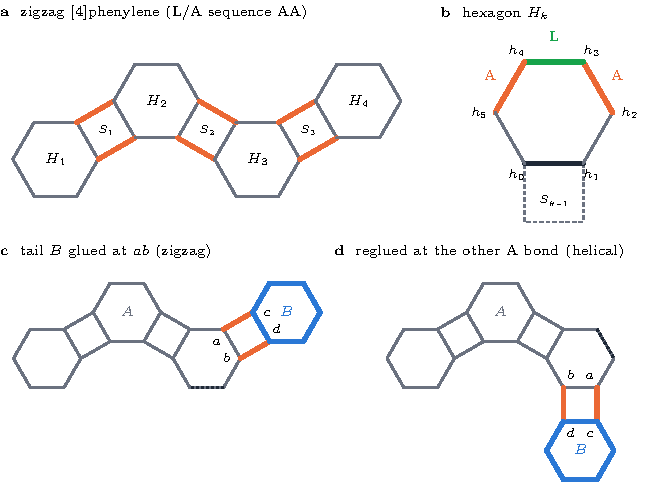
\includegraphics{fig_la.pdf}
\caption{Phenylenes and the gluing construction. (a) Zigzag [4]phenylene with its hexagons $H_k$ and four-membered rings $S_k$; the connecting bonds are orange. (b) An internal hexagon. The bond $h_0h_1$ is shared with the preceding ring $S_{k-1}$; the next ring $S_k$ is attached either at $h_3h_4$ (L) or at one of $h_2h_3$ and $h_4h_5$ (A). (c) Zigzag [4]phenylene split as in Lemma~\ref{lem:glue}: head $A$ (grey), tail $B$ (blue) and the connecting bonds $ac$ and $bd$ (orange). The dotted bond is the other angular bond of $H_3$. (d) The same tail glued at that bond gives helical [4]phenylene. Theorem~\ref{thm:la} shows that this move preserves the signed Kekul\'e polynomial.}
\label{fig:la}
\end{figure}

\begin{lemma}[Gluing formula]
\label{lem:glue}
Let $G$ consist of two disjoint bipartite graphs $A$ and $B$, each with an even number of atoms, together with two connecting bonds $ac$ and $bd$, where $ab$ is a bond of $A$ and $cd$ a bond of $B$. Write $P_X$ for the signed Kekul\'e polynomial of $X$ and $x_e$ for the variable of bond $e$. Then, up to an overall sign,
\begin{equation}
P_G=P_A\,P_B-x_{ac}\,x_{bd}\,\frac{\partial P_A}{\partial x_{ab}}\,\frac{\partial P_B}{\partial x_{cd}} .
\label{eq:glue}
\end{equation}
\end{lemma}

\begin{proof}
A Kekul\'e structure of $G$ contains either both connecting bonds or neither. Suppose it contained $ac$ but not $bd$. Then every atom of $A$ other than $a$ would have to be covered by double bonds inside $A$. These atoms are odd in number, and each double bond covers two of them, so this is impossible; the same argument applies to $bd$ alone. The structures without connecting bonds are the unions $M_A\cup M_B$ of structures of $A$ and $B$. Two such unions differ by cycles that lie in $A$ or in $B$, so by the rule of Dewar and Longuet-Higgins \citep{DewarLH1952} their relative sign is the product of the relative signs in $A$ and in $B$; these terms sum to $P_AP_B$. A structure with both connecting bonds is $N_1=\{ac,bd\}\cup M'_A\cup M'_B$, where $M'_A$ covers $A$ without $a,b$ and $M'_B$ covers $B$ without $c,d$. It differs from $N_0=\{ab,cd\}\cup M'_A\cup M'_B$, a structure without connecting bonds, by the single four-membered cycle $a\,b\,d\,c$, so $s_{N_1}=-s_{N_0}$. The terms of $P_AP_B$ that contain $x_{ab}x_{cd}$ are $x_{ab}x_{cd}\,\partial_{ab}P_A\,\partial_{cd}P_B$, and replacing $x_{ab}x_{cd}$ by $-x_{ac}x_{bd}$ in them gives the remaining terms of $P_G$.
\end{proof}

The tail of a phenylene enters Eq.~\eqref{eq:glue} only through $P_B$, $\partial_{cd}P_B$ and the product $x_{ac}x_{bd}$, and the head only through $P_A$ and the derivative with respect to the bond at which the tail is attached. The two angular positions of the last hexagon of the head give the same derivative up to relabelling.

\begin{lemma}
\label{lem:swap}
Let $A$ be a phenylene, or a single hexagon, whose last hexagon has atoms $h_0,\dots,h_5$ in cyclic order, where $h_0h_1$ is the bond shared with the preceding four-membered ring (any bond if $A$ is a single hexagon). Exchanging the variables of the bonds $h_2h_3$ and $h_4h_5$ leaves $P_A$ unchanged and turns $\partial P_A/\partial x_{h_2h_3}$ into $\partial P_A/\partial x_{h_4h_5}$.
\end{lemma}

\begin{proof}
The atoms $h_2,h_3,h_4,h_5$ lie only in the bonds of the path $h_1h_2h_3h_4h_5h_0$. A Kekul\'e structure covers them either by $h_2h_3$ and $h_4h_5$ together, or by $h_1h_2$, $h_3h_4$ and $h_5h_0$; it never contains exactly one of $h_2h_3$ and $h_4h_5$. Hence $P_A=x_{h_2h_3}x_{h_4h_5}R+S$, where $R$ and $S$ do not contain these two variables, and $\partial_{h_2h_3}P_A=x_{h_4h_5}R$, $\partial_{h_4h_5}P_A=x_{h_2h_3}R$.
\end{proof}

\begin{theorem}
\label{thm:la}
Two [$N$]phenylenes with the same L/A sequence, up to reversal, have the same signed Kekul\'e polynomial up to a one-to-one correspondence of their bonds and an overall sign. They therefore have the same number of Kekul\'e structures, the same algebraic structure count and, by Proposition~\ref{prop:inv}, the same closure threshold and the same upper bound $\bar\rho$.
\end{theorem}

\begin{proof}
Call a \emph{regluing} at $H_k$ the following move: cut the connecting bonds of $S_k$, so that the phenylene splits into a head $A$ (hexagons $H_1,\dots,H_k$) and a tail $B$ (the rest, with $H_{k+1}$ containing the bond $cd$), and attach $B$ again through two new connecting bonds, either at the same bond of $H_k$ with the opposite orientation or, if $H_k$ is angularly annelated, at the other angular bond. A regluing keeps the L/A sequence. It also keeps the signed Kekul\'e polynomial up to relabelling: map the bonds of $B$ to themselves, the bonds of $A$ to themselves except for exchanging $h_2h_3$ and $h_4h_5$ in the angular case, and each old connecting bond to the new connecting bond at the same atom of $B$. By Lemma~\ref{lem:swap} this map carries $P_A$ to itself and the derivative at the old attachment bond to the derivative at the new one, and Eq.~\eqref{eq:glue} does not depend on the orientation; so it carries $P_G$ onto $P_{G'}$.

Now let $G$ and $G'$ have the same L/A sequence, reading $G'$ backwards if necessary. Any two attachments of $S_1$ to $H_1$ are related by a symmetry of the hexagon, so $H_1\cup S_1\cup H_2$ in $G$ and in $G'$ correspond under a graph isomorphism. Suppose the first $k$ hexagons of $G$ and $G'$, with the rings between them, correspond under an isomorphism $\psi$. The attachment bond of $S_k$ in $G'$ and its image under $\psi^{-1}$ have the same annelation mode in $H_k$, so a regluing of $G$ at $H_k$ makes the first $k+1$ hexagons correspond. After $N-2$ regluings $G$ has become isomorphic to $G'$, and the composition of the bond maps is the required correspondence.
\end{proof}

Theorem~\ref{thm:la} extends the isoarithmicity of hexagonal chains \citep{GordonDavison1952,BalabanTomescu1983} from the number of Kekul\'e structures to the signed polynomial, with every coupling kept as a variable. For the algebraic structure count the statement also follows from the squeeze theorem \citep{Gutman1993} and isoarithmicity; the statements on $\rho$ and $\bar\rho$ need the polynomial and not only its value at equal couplings. The proof is constructive. For zigzag and helical [4]phenylene, a single regluing at $H_3$ suffices, and Appendix~\ref{app:corresp} lists the resulting bond correspondence; it fixes 26 of the 30 bonds. The theorem says nothing about the spectrum: helical and zigzag [4]phenylene have gaps of 0.703 and 0.743, and the [5]phenylenes with sequence AAA gaps between 0.672 and 0.727, each group with one threshold. We checked the theorem independently for all phenylenes with $N\le6$ (81 constructions for $N=6$, counting each choice of side separately) by testing the incidence structures of bonds and signed Kekul\'e structures for isomorphism.

% =====================================================================
\section{Thresholds and closing patterns of phenylenes}
\label{sec:phenylenes}

\subsection{Computing the threshold}

Poljak and Rohn showed that a finite set of $2^{2n}$ matrices decides the regularity radius \citep{PoljakRohn1993,HartmanHladik2018}. For sign vectors $y,z\in\{-1,1\}^n$, change each coupling $t_{ij}$ by $-\epsilon\,y_iz_j\,t_{ij}$. Along this family the determinant vanishes at $\epsilon=1/\lambda$ for each real eigenvalue $\lambda$ of $T^{-1}(T\circ yz^\T)$, where $\circ$ is the elementwise product, and
\begin{equation}
\rho=\Bigl[\max_{y,z}\ \lambda_{\mathbb R}\bigl(T^{-1}(T\circ yz^\T)\bigr)\Bigr]^{-1},
\label{eq:rohn}
\end{equation}
with $\lambda_{\mathbb R}$ the largest absolute value of a real eigenvalue. Fixing $z_1=1$ removes an overall sign and leaves $2^{2n-1}$ eigenvalue problems of size $n$.

The thresholds in Table~\ref{tab:rho} rest on three arguments, which establish different things:
\begin{enumerate}
\item \emph{Closed form.} For benzocyclobutadiene and biphenylene, Theorem~\ref{thm:one} gives $\rho$ as the root of a polynomial.
\item \emph{Complete enumeration.} For every skeleton, Eq.~\eqref{eq:rohn} is an exact characterization over a finite set, and we evaluate all $2^{2n-1}$ eigenvalue problems, up to $2^{23}$ for the [4]phenylenes. No search or sampling is involved.
\item \emph{Floating-point arithmetic.} The eigenvalues are computed in double precision with LAPACK, and an eigenvalue counts as real when its imaginary part is below $10^{-9}$. A second argument fixes every tabulated $\rho$ without this tolerance. Because $\det T$ is affine in each coupling, its minimum over $\Bx_\epsilon(T)$ is attained at a corner of the box, where each coupling equals $1+\epsilon$ or $1-\epsilon$. We evaluate the determinant at all $2^m$ corners through Eq.~\eqref{eq:expansion}, splitting the bonds into two halves so that the corner values become the entries of a matrix product. At $\epsilon=\rho(1-10^{-8})$ the smallest corner value is positive, at least $1.0\times10^{-8}$; at $\epsilon=\rho(1+10^{-8})$ it is negative. The rounding error of these sums is at most $10^{-12}$. Each tabulated $\rho$ is therefore correct to a relative error of $10^{-8}$, and the closed forms of Theorem~\ref{thm:one} agree with the computed values to $10^{-15}$.
\end{enumerate}

\begin{table}[t]
\centering
\caption{Closure thresholds. L/A: annelation sequence; $K$: number of Kekul\'e structures; ASC: algebraic structure count; $g$: H\"uckel gap at equal couplings; $\rho$: closure threshold; patterns: number of singular matrices in $\Bx_\rho(T)$; single bond: smallest change of one coupling that closes the gap while keeping that coupling positive (+, increase; $-$, decrease); none if no such change exists.}
\label{tab:rho}
\begin{tabular}{llrrrrrrr}
\toprule
skeleton & L/A & atoms & $K$ & ASC & $g/|\beta|$ & $\rho$ & patterns & single bond \\
\midrule
benzene & & 6 & 2 & 2 & 2.000 & 1 & -- & none \\
naphthalene & & 10 & 3 & 3 & 1.236 & 1 & -- & none \\
benzocyclobutadiene & & 8 & 3 & 1 & 0.525 & 0.1197 & 1 & $-50\%$ \\
biphenylene & -- & 12 & 5 & 3 & 0.890 & 0.1888 & 1 & $+300\%$ \\
linear [3]phenylene & L & 18 & 12 & 4 & 0.525 & 0.1197 & face$^{a}$ & $+200\%$ \\
angular [3]phenylene & A & 18 & 13 & 5 & 0.844 & 0.1962 & 2 & $+500\%$ \\
linear [4]phenylene & LL & 24 & 29 & 5 & 0.348 & 0.0756 & 1 & $-83\%$ \\
bent [4]phenylene & LA & 24 & 31 & 7 & 0.565 & 0.1265 & 1 & $+233\%$ \\
helical [4]phenylene & AA & 24 & 34 & 8 & 0.703 & 0.1614 & 1 & $+400\%$ \\
zigzag [4]phenylene & AA & 24 & 34 & 8 & 0.743 & 0.1614 & 1 & $+400\%$ \\
triangular [4]phenylene & & 24 & 35 & 9 & 0.905 & 0.2031 & 3 & $+900\%$ \\
\bottomrule
\end{tabular}

\smallskip
{\footnotesize $^{a}$A four-dimensional face of the box with 16 corners (Section~\ref{sec:patterns}).}
\end{table}

Complete enumeration matters in practice. A search that starts from random sign vectors and flips one sign at a time until Eq.~\eqref{eq:rohn} stops improving returns 0.1666 for zigzag [4]phenylene, above the exact value 0.1614. This value coincides with the upper bound $\bar\rho$ of Proposition~\ref{prop:bounds} to 15 digits: the search stalls at the corner of a single minority structure.

\subsection{Thresholds across skeletons}

Table~\ref{tab:rho} lists the thresholds for the [$N$]phenylenes with $N\le4$. Every phenylene closes with a change of 7.6\% to 20.3\%, while the single-bond route needs a coupling to grow severalfold or to shrink to half or less. Along the linear series the threshold falls from 18.9\% to 12.0\% to 7.6\%, in the same direction as the rising reactivity and red shift of linear phenylenes \citep{Vollhardt1993,Dosche2002}. This trend reflects the infinite chain. At equal couplings the linear phenylene polymer has no gap: its highest occupied band reaches zero energy at wave vector $k=0$ and its lowest unoccupied band at $k=\pi$. The gaps of finite linear chains accordingly fall as $1/N^2$, with $N^2g$ reaching 9.75 at $N=160$, close to $\pi^2$, and the upper bound $\bar\rho$ of Table~\ref{tab:bounds} decreases along the series L, LL, LLL, LLLL. Angular chains behave differently: zigzag and helical chains with $N=40$ still have gaps of 0.58 and 0.50. Angular and branched skeletons need larger changes than linear ones of the same size. What fixes $\rho$ is the full list of signed Kekul\'e structures, and two simpler quantities capture only part of it. Biphenylene and naphthalene, its hexagonal squeeze, have the same algebraic structure count, three; but all Kekul\'e structures of naphthalene carry one sign, so its threshold is 1, against 0.189 for biphenylene. Angular [3]phenylene has a smaller gap than biphenylene and a larger threshold. Helical and zigzag [4]phenylene, which share their signed Kekul\'e structures by Theorem~\ref{thm:la}, have gaps of 0.703 and 0.743 and the same threshold.

Table~\ref{tab:bounds} compares the bounds of Proposition~\ref{prop:bounds} with $\rho$, grouped by L/A sequence. Theorem~\ref{thm:la} allows the lower bound of a sequence to be taken as the largest $\underline\rho$ among its phenylenes, since they share $\rho$; this matters for the gap bound, which differs between them. The upper bound is attained for biphenylene and lies within 0.4\% of $\rho$ for angular [3]phenylene, 0.8\% for triangular [4]phenylene and 3\% for the sequence AA. It is loose for linear chains: 0.160 against 0.120 for L and 0.125 against 0.076 for LL. In linear phenylenes the closing pattern is not the corner of one minority structure but a combination of several, and Section~\ref{sec:patterns} shows that it is spread over the whole chain. For $N=5$ and 6, where exact enumeration is out of reach, the bounds bracket $\rho$ for all 16 L/A sequences at a cost of one eigenvalue problem per phenylene and one polynomial root per minority structure.

\begin{table}[t]
\centering
\caption{Bounds on the closure threshold by L/A sequence (sequences read in either direction are listed once). $g$: range of H\"uckel gaps over all phenylenes with the sequence; $\underline\rho$: largest lower bound of Proposition~\ref{prop:bounds}(a) over these phenylenes; $\bar\rho$: upper bound of Proposition~\ref{prop:bounds}(b); $\rho$: exact value (Table~\ref{tab:rho}).}
\label{tab:bounds}
\small
\begin{tabular}{rlrrcccc}
\toprule
$N$ & L/A & $K$ & ASC & $g/|\beta|$ & $\underline\rho$ & $\rho$ & $\bar\rho$ \\
\midrule
2 & --   & 5   & 3  & 0.890       & 0.1758 & 0.1888 & 0.1888 \\
3 & L    & 12  & 4  & 0.525       & 0.0996 & 0.1197 & 0.1598 \\
3 & A    & 13  & 5  & 0.844       & 0.1584 & 0.1962 & 0.1970 \\
4 & LL   & 29  & 5  & 0.348       & 0.0651 & 0.0756 & 0.1248 \\
4 & LA   & 31  & 7  & 0.565       & 0.1048 & 0.1265 & 0.1619 \\
4 & AA   & 34  & 8  & 0.703--0.743 & 0.1367 & 0.1614 & 0.1666 \\
5 & LLL  & 70  & 6  & 0.249       & 0.0474 & & 0.1152 \\
5 & LLA  & 75  & 9  & 0.383       & 0.0707 & & 0.1287 \\
5 & LAL  & 74  & 10 & 0.546       & 0.1006 & & 0.1624 \\
5 & LAA  & 81  & 11 & 0.503--0.510 & 0.0934 & & 0.1503 \\
5 & ALA  & 80  & 12 & 0.594--0.603 & 0.1108 & & 0.1731 \\
5 & AAA  & 89  & 13 & 0.672--0.727 & 0.1324 & & 0.1724 \\
6 & LLLL & 169 & 7  & 0.186       & 0.0363 & & 0.0769 \\
6 & LLLA & 181 & 11 & 0.275       & 0.0506 & & 0.1165 \\
6 & LLAL & 179 & 13 & 0.392       & 0.0720 & & 0.1295 \\
6 & LLAA & 196 & 14 & 0.354--0.355 & 0.0650 & & 0.1197 \\
6 & LAAL & 193 & 15 & 0.421--0.427 & 0.0780 & & 0.1321 \\
6 & ALLA & 194 & 16 & 0.417--0.418 & 0.0767 & & 0.1321 \\
6 & LALA & 191 & 17 & 0.539--0.553 & 0.1012 & & 0.1613 \\
6 & LAAA & 212 & 18 & 0.512--0.523 & 0.0950 & & 0.1576 \\
6 & ALAA & 209 & 19 & 0.532--0.544 & 0.0992 & & 0.1517 \\
6 & AAAA & 233 & 21 & 0.624--0.685 & 0.1243 & & 0.1575 \\
\bottomrule
\end{tabular}
\end{table}

\subsection{Closing patterns and closing orbitals}
\label{sec:patterns}

We call a singular matrix in $\Bx_\rho(T)$ a \emph{closing pattern}. Theorem~\ref{thm:one} identifies the closing pattern of benzocyclobutadiene and biphenylene and proves that it is unique. For the other skeletons we find all closing patterns by computation, using the following consequence of the affine dependence on each coupling.

\begin{lemma}
\label{lem:corner}
Suppose that no two singular corners of $\Bx_\rho(T)$ differ in a single coupling. Then every closing pattern is a corner of $\Bx_\rho(T)$.
\end{lemma}

\begin{proof}
Below $\rho$ the box contains no singular matrix, so $\det T'\ge0$ on $\Bx_\rho(T)$ and closing patterns are minimizers of $\det T'$. Let $T'$ be a closing pattern with some coupling strictly inside its interval. Along this coupling $\det$ is affine and has an interior minimum, so it is constant, and both endpoints give closing patterns. Moving the remaining interior couplings of both matrices to the same endpoints, one at a time and by the same argument, yields two singular corners that differ in this coupling only.
\end{proof}

To find all closing patterns, we evaluate $\det T$ at the $2^m$ corners of $\Bx_\rho(T)$ in the same way as for the values in Table~\ref{tab:rho}. The singular corners are well separated from the others: their determinants are below $10^{-13}$, while every other corner gives at least 0.03. Their numbers are listed in Table~\ref{tab:rho}. For every skeleton except linear [3]phenylene no two singular corners are adjacent, so by Lemma~\ref{lem:corner} these corners are all the closing patterns. Each of them is of the sign-vector form $T-\rho\,T\circ yz^\T$ up to the sign of the change, so Eq.~\eqref{eq:rohn} finds every one of them.

At a closing pattern $T$ has left and right null vectors $\phi$ and $\psi$, one on each set of atoms. They define the \emph{closing orbital}, the pair of orbitals that reach zero energy; atom $i$ carries weight $\phi_i^2/2$ on one set and $\psi_j^2/2$ on the other. Figure~\ref{fig:where} shows these weights for six phenylenes.

\begin{figure}[tbp]
\centering
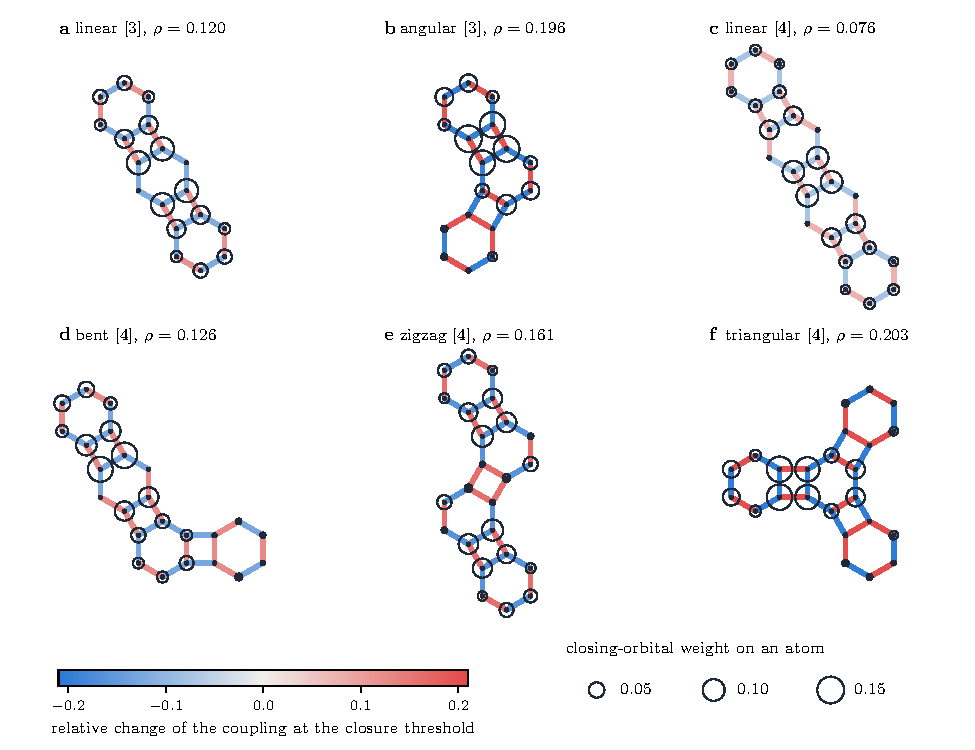
\includegraphics{fig2_closing.pdf}
\caption{Closing patterns and closing orbitals of six [$N$]phenylenes, drawn to a common scale. Bond colour: relative change of the coupling at the closure threshold (red, stronger; blue, weaker). Circle area: weight of the closing orbital on each atom.}
\label{fig:where}
\end{figure}

The annelation pattern determines where on the skeleton the gap closes. In linear phenylenes the closing orbital spreads along the whole chain, with its weight peaking at the centre. In angular and branched skeletons it concentrates at one end. In angular [3]phenylene one terminal benzene--cyclobutadiene--benzene unit carries 90\% of the weight; in bent [4]phenylene one terminal unit carries 68\%; in triangular [4]phenylene the central ring and one arm carry 82\%. In zigzag and helical [4]phenylene the two terminal units carry nearly all of it and the central four-membered ring 2\%. Because the list of closing patterns is complete, this localization is a property of the skeletons themselves. Angular [3]phenylene has exactly two closing patterns, mirror images of each other, which close the gap at opposite ends. Triangular [4]phenylene has three, one on each arm, related by the threefold rotation. Bent, zigzag and helical [4]phenylene have one each. In every angular or branched skeleton, each closing pattern is confined to one part of the molecule. The bounds of Table~\ref{tab:bounds} reflect the same fact: where the gap closes locally, strengthening a single minority structure comes within a few per cent of the threshold.

Linear [3]phenylene behaves differently. It has 16 singular corners, some of which differ in a single coupling, so Lemma~\ref{lem:corner} does not apply. Its threshold and its gap both equal those of benzocyclobutadiene (Table~\ref{tab:rho}), and a symmetry explains why. The mirror plane perpendicular to the long axis passes through two atoms of the central benzene ring, the two that do not belong to a four-membered ring; call them the mirror atoms. An orbital that is antisymmetric under this mirror has zero amplitude on the mirror atoms. For such orbitals the molecule falls apart into its two halves, and each half is benzocyclobutadiene. Applying the closing pattern of benzocyclobutadiene to both halves therefore closes the gap of linear [3]phenylene, which proves $\rho_{\text{lin-3}}\le\rho_{\text{BCB}}$; the computation gives equality.

The 16 singular corners have a simple structure. They agree in every coupling except the four couplings of the bonds that touch the mirror atoms, and these four take all $2^4=16$ combinations of $1-\rho$ and $1+\rho$. In other words, the singular corners are the corners of one four-dimensional face of the box. On this face $\det T$ is affine in each of the four free couplings and vanishes at every corner, so it vanishes on the whole face. The argument in the proof of Lemma~\ref{lem:corner} shows that no singular matrix lies outside the face. The closing patterns of linear [3]phenylene are therefore exactly the points of this face: once the other couplings are set, the four couplings at the mirror atoms can take any allowed values.

% =====================================================================
\section{Application: closure energy in a bond-length model}
\label{sec:energy}

A molecule changes its couplings by changing bond lengths, and bond lengths resist. We let each coupling depend on the change $\delta_b$ of its bond length from a common reference, $t_b=t_0-\alpha\,\delta_b$, and add a harmonic $\sigma$ energy \citep{SSH1979}:
\begin{equation}
E(\delta)=-2\sum_k\sigma_k\bigl(T(\delta)\bigr)+\sum_b\Bigl(\tfrac{f_\sigma}{2}\delta_b^2+c\,\delta_b\Bigr),\qquad c=-2\alpha p_{\text{ref}},
\end{equation}
with $p_{\text{ref}}=2/3$, so that benzene is undistorted at $\delta=0$, $t_0=2.5$~eV, $\alpha=4.1$~eV\,\AA$^{-1}$ \citep{SSH1979} and $f_\sigma=43$~eV\,\AA$^{-2}$ (Appendix~\ref{app:model}). The \emph{closure energy} $\Delta E$ is the lowest energy on the set of geometries with $\det T(\delta)=0$, measured from the relaxed geometry. It ranges from 1.9~eV for linear [4]phenylene to 5.5~eV for triangular [4]phenylene (Table~\ref{tab:cost}).

The threshold and the closure energy answer different optimization problems: $\rho$ minimizes the largest relative change of a coupling and contains no energy, while $\Delta E$ minimizes an energy over bond lengths. Still, $\rho$ ranks the nine closure energies with Spearman correlation 0.94, while the gap of the relaxed geometry ranks them with 0.72. The local quadratic approximation explains why. With $x$ the vector of bond-length changes from the relaxed geometry, $\gamma$ the gradient of the gap and $F$ the Hessian of the energy, minimizing $\tfrac12x^\T Fx$ subject to $g_0+\gamma^\T x=0$ gives
\begin{equation}
\Delta E\approx\frac{g_0^2}{2\,\gamma^\T F^{-1}\gamma},\qquad x^*=-\frac{g_0\,F^{-1}\gamma}{\gamma^\T F^{-1}\gamma}.
\label{eq:local}
\end{equation}
If $u$ and $v$ are the singular vectors of the relaxed $T$ for $\sigma_{\min}$, then $\partial g/\partial t_{ij}=2u_iv_j$, and $u_iv_j=p^{\mathrm{H}}_{ij}-p^{\mathrm{L}}_{ij}$ is the difference between the HOMO and LUMO partial bond orders \citep{CoulsonLH1947}. With
\begin{equation}
P=\sum_{(ij)}\bigl(p^{\mathrm{H}}_{ij}-p^{\mathrm{L}}_{ij}\bigr)^2
\label{eq:P}
\end{equation}
we have $\gamma^\T\gamma=4\alpha^2P$. The Hessian combines the $\sigma$ springs with the bond--bond polarizability \citep{CoulsonLH1947,BHM1966}, to which the HOMO--LUMO pair contributes nothing by the pairing theorem \citep{CoulsonRushbrooke1940,FowlerRassat2002}; its eigenvalues lie between 27.9 and 43.0~eV\,\AA$^{-2}$ for all nine skeletons. With $F\approx\bar f\,I$, Eq.~\eqref{eq:local} becomes $\Delta E\approx(\bar f/8\alpha^2)\,g_0^2/P$. Biphenylene has a larger gap than angular [3]phenylene, 2.58 against 2.39~eV, but its frontier orbitals concentrate on fewer bonds ($P=0.45$ against $0.27$), and its gap closes for 4.18 instead of 4.77~eV.

\begin{table}[t]
\centering
\caption{Closure energy in the bond-length model ($f_\sigma=43$~eV\,\AA$^{-2}$). $\rho$: closure threshold (Table~\ref{tab:rho}); $g_0$: gap of the relaxed geometry; $P$: Eq.~\eqref{eq:P}; $\Delta E_{\text{loc}}$: Eq.~\eqref{eq:local}; $\Delta E$: lowest closure energy found. Last rows: Spearman rank correlation with $\Delta E$ and its two-sided $p$ value from the exact permutation distribution (all $9!$ orderings; ties as mid-ranks).}
\label{tab:cost}
\begin{tabular}{lrrrrrr}
\toprule
skeleton & $\rho$ & $g_0$ (eV) & $P$ & $g_0^2/P$ & $\Delta E_{\text{loc}}$ (eV) & $\Delta E$ (eV) \\
\midrule
linear [4]phenylene & 0.076 & 1.35 & 0.268 & 6.79 & 1.93 & 1.87 \\
benzocyclobutadiene & 0.120 & 2.09 & 0.644 & 6.78 & 2.00 & 2.01 \\
linear [3]phenylene & 0.120 & 1.75 & 0.326 & 9.37 & 2.67 & 2.70 \\
bent [4]phenylene & 0.126 & 1.77 & 0.282 & 11.16 & 3.11 & 3.05 \\
biphenylene & 0.189 & 2.58 & 0.449 & 14.87 & 4.31 & 4.18 \\
helical [4]phenylene & 0.161 & 2.08 & 0.212 & 20.40 & 5.49 & 4.51 \\
zigzag [4]phenylene & 0.161 & 2.20 & 0.229 & 21.22 & 5.93 & 4.52 \\
angular [3]phenylene & 0.196 & 2.39 & 0.274 & 20.83 & 5.63 & 4.77 \\
triangular [4]phenylene & 0.203 & 2.48 & 0.226 & 27.34 & 7.48 & 5.55 \\
\midrule
Spearman with $\Delta E$ & 0.94 & 0.72 & & 0.97 & 0.98 & \\
$p$ & $5.5\times10^{-4}$ & 0.037 & & $1.7\times10^{-4}$ & $5.0\times10^{-5}$ & \\
\bottomrule
\end{tabular}
\end{table}

We call $x^*$ the predicted pattern and compared its direction with B3LYP in the def2-SVP basis for biphenylene and angular [3]phenylene (Appendix~\ref{app:dft}). For this we computed the gradient $\gamma_{\mathrm B}$ of the Kohn--Sham gap with respect to the C--C bond lengths by finite differences. At a given model energy, the B3LYP gap falls fastest along $-F^{-1}\gamma_{\mathrm B}$, just as the model gap falls fastest along $x^*\propto-F^{-1}\gamma$. The cosine between these two directions, measured in the metric of $F$, is 0.989 for both molecules; for the random bond-length patterns of Appendix~\ref{app:dft} the median is 0.17 and 0.13. The pattern derived from the H\"uckel model is therefore almost the steepest-descent direction of the B3LYP gap. Along it, the gap also falls 2.4 and 3.6 times more per eV of B3LYP deformation energy than when the bond-length alternation is undone.

% =====================================================================
\section{Discussion}

How robust is an open H\"uckel gap? For phenylenes and related skeletons, the answer can be read from the signed Kekul\'e structures. The closure threshold depends on nothing else, and it equals 1, its largest value, exactly when all structures carry one sign. Three results show how the structures determine it. When one structure carries the minority sign, the numbers $k_a$ by which the other structures differ from it fix the threshold through $\sum_aq^{k_a}=1$; in biphenylene the exponents 2, 4, 4, 6 give $q^3+q=1$ and a threshold of 18.9\%. In general, strengthening one minority structure bounds the threshold from above, and the bound is close when closure is local. For phenylenes, the polynomial and hence the threshold depend only on the L/A sequence, so the threshold is an invariant of the sequence in the same sense as the Kekul\'e count of a hexagonal chain.

The cooperative changes that close the gap are also small in chemical terms. With couplings linear in bond length, as in Section~\ref{sec:energy}, a change of 18.9\% in every coupling of biphenylene corresponds to at most 0.12~\AA\ per bond, comparable to ordinary bond-length alternation. Closing the gap through one bond instead requires its coupling to grow fourfold, which in the same model means shortening that bond by 1.8~\AA, more than its own length; the bond-length model puts the cost of this route at 113~eV, against 4.2~eV for the cooperative one.

Chemically, the most interesting regime lies before the gap closes. Along the bond-length pattern of Section~\ref{sec:energy}, the B3LYP singlet of biphenylene and of angular [3]phenylene acquires open-shell character while the gap is still about 2~eV. The threshold therefore measures the distance to the end point of a path along which diradical character grows, as it does in polycyclic hydrocarbons with four-membered rings \citep{MolesQuintero2022}.

Several questions follow. Exact computation of $\rho$ is exponential in the number of atoms, and Proposition~\ref{prop:bounds} brackets it cheaply; a lower bound that, like $\bar\rho$, uses the Kekul\'e structures would close the bracket for linear chains, where the spectral bounds and $\bar\rho$ are furthest apart. Theorem~\ref{thm:one} covers every skeleton with one minority structure, and it would be useful to know which skeletons these are. The gluing formula, Eq.~\eqref{eq:glue}, applies to any two bipartite graphs joined through a four-membered ring, so the argument of Theorem~\ref{thm:la} may extend to branched phenylenes and to other chains of benzenoid units joined by four-membered rings.

% =====================================================================
\appendix
\section{Bond-length model}
\label{app:model}

\begin{center}
\small
\begin{tabular}{lll}
\toprule
parameter & symbol & value \\
\midrule
coupling at the reference length & $t_0$ & 2.5~eV \\
decrease of coupling per \AA & $\alpha$ & 4.1~eV\,\AA$^{-1}$ \\
$\sigma$ force constant & $f_\sigma$ & 43~eV\,\AA$^{-2}$ (also 21 and 60) \\
reference bond order & $p_{\text{ref}}$ & 2/3 \\
\bottomrule
\end{tabular}
\end{center}

At equilibrium $\delta_b=2\alpha(p_{\text{ref}}-p_b)/f_\sigma$, which at $f_\sigma=43$~eV\,\AA$^{-2}$ is a slope of 0.19~\AA\ per unit bond order.

\textbf{Relaxed geometries} were found by BFGS minimization from $\delta=0$. Relaxation widens the gap in all nine skeletons.

\textbf{Closure energies} were found by sequential quadratic programming under the constraint that $\det T(\delta)$ vanishes, scaled by $t_0^{-n}$; its gradient follows from the adjugate. The starting points were the closing pattern of Eq.~\eqref{eq:rohn}, the relaxed geometry plus multiples of it, and random perturbations of the relaxed geometry; we report the lowest feasible result.

\textbf{Dependence on $f_\sigma$.} At $f_\sigma=21$, 43 and 60~eV\,\AA$^{-2}$ the closure energies range over 1.7--2.9, 1.9--5.5 and 2.2--7.7~eV, and they rank the nine skeletons in the same order.

\textbf{Accuracy of Eq.~\eqref{eq:local}.} The local approximation reproduces $\Delta E$ within 5\% for benzocyclobutadiene, biphenylene, the linear skeletons and bent [4]phenylene. It overestimates $\Delta E$ by 18--35\% for the angular and branched skeletons, whose closures lie farthest from the relaxed geometry.

\textbf{Degenerate frontier level.} In triangular [4]phenylene the relaxed frontier level is doubly degenerate. There $\gamma$ in Eq.~\eqref{eq:local}, and likewise $P$, is taken in the direction of the two-dimensional frontier subspace that maximizes $\gamma^\T F^{-1}\gamma$.

\section{Bond correspondence of zigzag and helical [4]phenylene}
\label{app:corresp}

\begin{figure}[h]
\centering
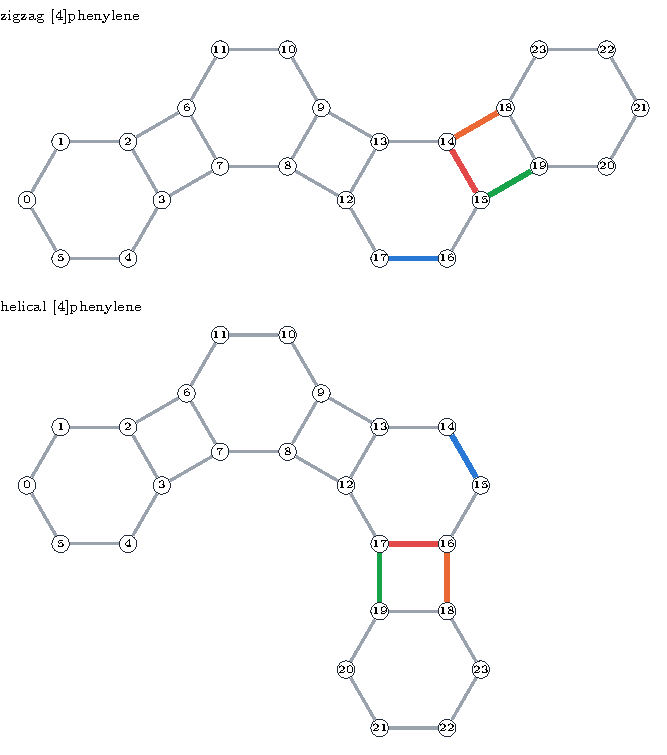
\includegraphics{fig_corresp.pdf}
\caption{Atom numbering of zigzag and helical [4]phenylene. Bonds of the same colour correspond to each other; every grey bond corresponds to the bond with the same atom labels in the other skeleton.}
\label{fig:corresp}
\end{figure}

With the atom numbering of Fig.~\ref{fig:corresp}, the regluing at the third hexagon in the proof of Theorem~\ref{thm:la} maps every bond of zigzag [4]phenylene to the bond with the same atom labels in helical [4]phenylene, except for four bonds:
\begin{center}
\begin{tabular}{ll}
\toprule
zigzag [4]phenylene & helical [4]phenylene \\
\midrule
(14,15) & (16,17) \\
(16,17) & (14,15) \\
(14,18) & (16,18) \\
(15,19) & (17,19) \\
\bottomrule
\end{tabular}
\end{center}
The first two rows exchange the two angular bonds of the third hexagon (Lemma~\ref{lem:swap}); the last two map the connecting bonds of the last four-membered ring. Both signed Kekul\'e polynomials have 34 terms, 13 of them negative at equal couplings, and expanding both confirms that the correspondence maps each term of one onto a term of the other with the same sign. The correspondence is not induced by a map of atoms; the two skeletons are not isomorphic as graphs.

\section{B3LYP calculations}
\label{app:dft}

All calculations used B3LYP/def2-SVP \citep{Becke1993,LYP1988,WeigendAhlrichs2005} with density fitting in PySCF 2.14 \citep{PySCF2020}; geometries were optimized with pyberny. The equilibrium Kohn--Sham gaps are 4.10~eV (biphenylene) and 3.75~eV (angular [3]phenylene). Three kinds of bond-length change were applied, all scaled to the same model energy $\tfrac12x^\T Fx$: the predicted pattern $x^*$; a bond-equalizing control that undoes the bond-length alternation of the relaxed model geometry; and eight random patterns, each with both signs. Bond-length changes were converted to in-plane Cartesian displacements of the carbon atoms with the Wilson $B$ matrix \citep{Wilson1955}, hydrogens following their carbons. With fewer C--C bonds than in-plane carbon coordinates the solution is not unique; we took the minimum-norm least-squares solution and iterated it to convergence, so that the bond-length changes match their targets to $10^{-15}$~\AA. The bond angles adjust, and their strain enters the B3LYP energy. Displaced geometries were single points. Deformation energies are differences of restricted energies, and the gap is the Kohn--Sham gap of the restricted solution. The broken-symmetry singlet, converged from a HOMO--LUMO mixing guess and from the lower UHF solution, lies below the restricted one only beyond a model energy of 1.5~eV, by at most 0.02~eV at 2~eV. Spin symmetry breaking was taken as $\langle S^2\rangle>0.1$ in the broken-symmetry UB3LYP singlet.

\textbf{Gap gradient.} The gradient $\gamma_{\mathrm B}$ was computed by central differences, changing one C--C bond length at a time by $\pm0.005$~\AA\ with the same displacement scheme (28 single points for biphenylene, 44 for angular [3]phenylene, SCF convergence $10^{-10}$~hartree). Derivatives of symmetry-equivalent bonds of biphenylene agree to 0.001~eV\,\AA$^{-1}$. The cosine reported in Section~\ref{sec:energy} is
\[
\cos_F=\frac{\gamma^\T F^{-1}\gamma_{\mathrm B}}{\sqrt{\gamma^\T F^{-1}\gamma}\,\sqrt{\gamma_{\mathrm B}^\T F^{-1}\gamma_{\mathrm B}}},
\]
the fraction of the largest possible first-order decrease of the B3LYP gap, at a given model energy, that $x^*$ achieves. It is 0.989 for both molecules; the ordinary cosine between $\gamma$ and $\gamma_{\mathrm B}$ is 0.990 and 0.989. The first-order description holds over the range used: at a model energy of 0.5~eV along $x^*$, $\gamma_{\mathrm B}$ predicts gap decreases of 1.01 and 0.89~eV, and the computed decreases are 1.02 and 0.87~eV.

\textbf{Efficiency.} The efficiency $\eta$ is the gap decrease per eV of B3LYP deformation energy (Fig.~\ref{fig:dft}). At a model energy of 1.5~eV, $\eta=1.27$ for $x^*$ in biphenylene, against 0.52 for the bond-equalizing control and a median of 0.23 over the random patterns, each taken with its better sign; in angular [3]phenylene the values are 1.10, 0.31 and 0.17. No random pattern reaches half the efficiency of $x^*$. For a response that does not prefer any direction, the best possible pattern would beat the median of eight random ones by factors of about 5.3 and 6.7 in 14 and 22 dimensions. The measured factors for $x^*$, 5.5 and 6.6, reach this ceiling, as expected from a cosine close to 1.

\begin{figure}[h]
\centering
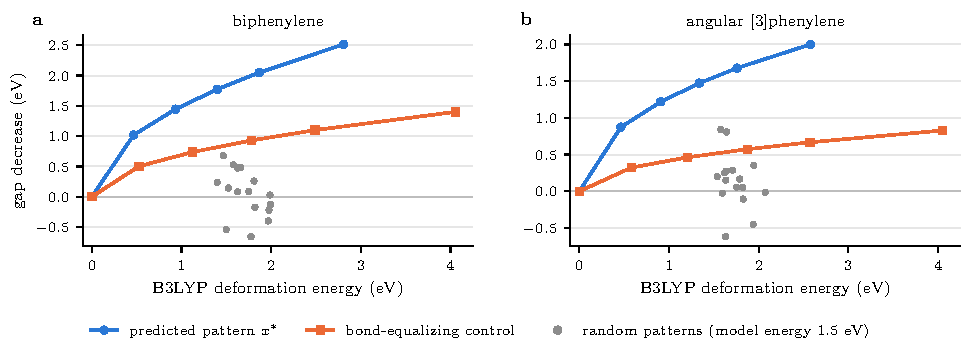
\includegraphics{fig3_dft_2panel.pdf}
\caption{Decrease of the Kohn--Sham gap against B3LYP deformation energy for the predicted pattern $x^*$, the bond-equalizing control and the random patterns (model energy 1.5~eV) in (a) biphenylene and (b) angular [3]phenylene.}
\label{fig:dft}
\end{figure}

\section*{Statements and Declarations}

\paragraph{Funding} No funds, grants, or other financial support were received for this study.

\paragraph{Competing interests} The author declares no relevant financial or non-financial competing interests.

\paragraph{Author contributions} Xiyao Yu conceived the study, developed the mathematical framework, performed the analytical and computational investigations, analyzed the results, and wrote and revised the manuscript.

\paragraph{Data and code availability} The source code, computational results, and data underlying all figures are publicly available at \url{https://github.com/PillowSoprano/phenylene-gap-closure}. An archived snapshot (release v1.1.0) is available at Zenodo, \url{https://doi.org/10.5281/zenodo.23448791}. The code is released under the MIT License, and the data and figures under CC BY 4.0.

\paragraph{Ethics approval} Not applicable. This study involved theoretical analysis and computational simulations and did not involve human participants or animals.

\bibliographystyle{unsrtnat}
\bibliography{refs}

\end{document}
